\chapter{Generation of transferable knowledge}\label{ch:knowledge}

\epigraph{\textit{Science never solves a problem without creating ten more}}{George Bernard Shaw}

This last chapter conducts some final thoughts about my bachelor thesis.

Building the model was not an easy task. For the training, I needed to rent a cloud computing system from Amazon AWS \footnote{https://aws.amazon.com/de/}, otherwise my computer would have needed too long. Without renting a high power graphics card, the training process would have taken around 30 hours on my personal computer. I paid around 12\$ for 10 hours of GPU (graphics card) power. With this rented power, the training process only took around 3 hours. 

The predictions from the last Section \ref{ss:eval} showed that the generated summaries could be much more accurate. There are multiple ways to further enhance the quality of the generated summaries with the following approaches. 

\section{Improving the models performance} 

\subsection{First option}
Increasing the training data. The entire dataset consists of 568.454 training data rows. For my prototype I only limited my training to 250.000 rows. Even that I took only half of the available training data, the strong Amazon AWS GPU still took 3 hours to train the model. The computation time rises monotonically with the provided training data, so if I had used all of the available data, the entire process would have taken around 7 hours. 

It is not guaranteed that the quality of predicted summaries increases by using more training data, but this is by far the easiest screw to set for trying to improve the quality.

\subsection{Second option}
I already used the advanced version of the Recurrent Neural Network, the LSTM. But even the LSTM can be already outdated by way more advanced time-series cells. One possible example is the Bidirectional LSTM. Using bidirectional will use the inputs in two ways. One from the past to future and one from the future to past. The Bidirectional LSTM is capable of preserving information from both the future words and the past words. This cell can understand context much better than the usual LSTM. Still, this is very complicated to implement and this exceeded my time limitation for this thesis.

\subsection{Third option}
Using the Beam-Search strategy from Section \ref{ss:abstractive} can lead to better results. It starts by generating the first word, and keeps the 10 next most suitable sequences of words (beams) around and generates on top of them. But the generated words sometimes lack diversity. It needs to be tested whether the generated summaries have a higher quality with or without Beam-Search, but it is still worth a try. 


\subsection{Fourth option}

Taken from the Section \ref{ss:neuralgen} \textit{Combinational Approach} of the advanced techniques.

Pointer Generator Networks from Section \ref{ss:neuralgen} can improve the model's performance dramatically. Those networks build further on top of the attention layer. If we consider Figure \ref{used_methods}, the Pointer Generator Network would be right after attention. The same way Sequence to Sequence models are needed for applying the attention layer, the attention layer is needed for implementing the Pointer Generator. 

This is by far the most complicated option of those four, but the most state-of-the-art and the most promising one. 

\begin{figure}
	\begin{center}
		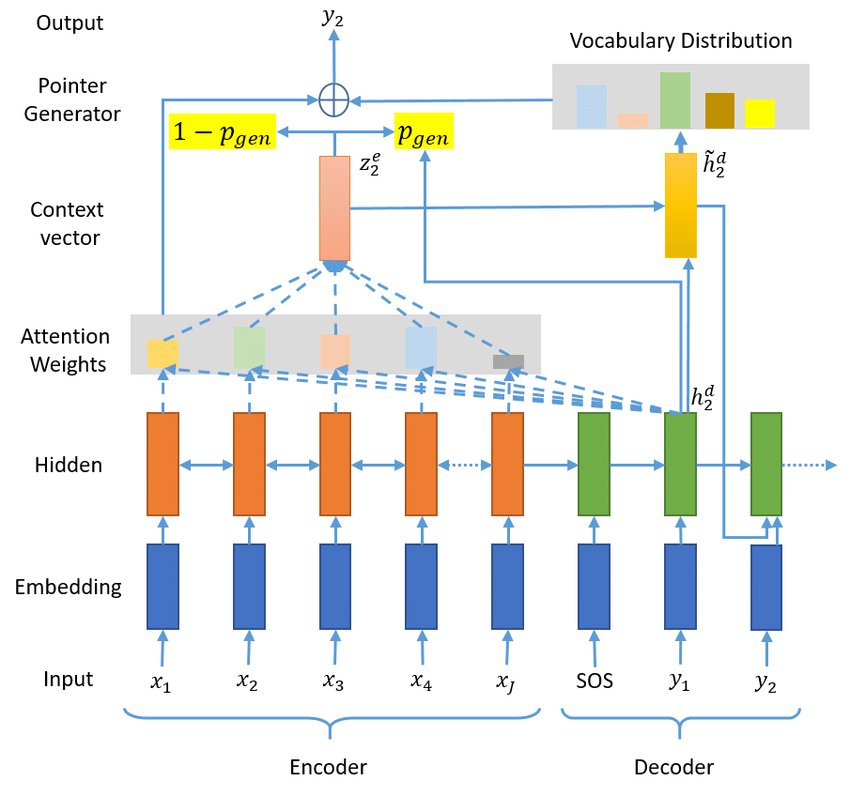
\includegraphics[width=3.5in]{photos/pgn}\\
		\caption{Pointer Generator Network architecture from \textit{https://www.researchgate.net/}}\label{pgn}
	\end{center}
\end{figure}

Figure \ref{pgn} shows a comparison between the attention architecture in Figure \ref{attention1} and the Pointer Generator Network. It shows the the architecture get further expanded on top attention. It is a hybrid network that can choose to copy words from the source via pointing, while at the same time allowing to retain generating words from our fixed vocabulary. 

\subsection{Fifth option}

Taken from the Section \ref{ss:neuralgen2} \textit{Transfer Learning Approach} of the advanced techniques.

Using Googles BERT architecture is an entirely different approach. Since Google uses this approach to summarize its own news headlines, it obviously also works very well for my task. Still, this architecture works differently and the prototype needs to be structured in another way. For the sake of my prototype I stayed with the basic sequence to sequence, to better explain how this easy architecture works.

I would be interesting to see how BERT is doing in summarizing the food reviews.

\section{Final Thoughts}

Making changes like the improvement tips in the model architecture requires much knowledge, so the most comfortable but most expensive way is increasing the training data size first. It was a though task for me to fully understand what my prototype is doing in depth, for that reason I kept it as simple as possible. The other highly research topics are more applicable for a master thesis. Even that the summaries are beyond not perfect, I am still proud that they show a certain level of intelligence. 


It made much fun to write this thesis and I learned so much new while investigating through text generation and text summarization. There is much more to explore and the Natural Language processing field is huge. 

The name for my thesis was at first \textit{IT-based Text Generation with the use of NLP Methods}. I noticed after the research that this title is not specific enough. Even in the range of Text Generation exist so many application fields, that the range I was searching in was just too wide. I decided to further decrease the scope of my thesis to be only about text summarization itself, but even that is probably not specific enough. 

It is interesting to see how specific something becomes after digging deep into the research material.

This project can be cloned from Github under the following link: \\ \\

\begin{tcolorbox}
	https://github.com/Mavengence/Bachelor-Thesis-Textgeneration-TH.OHM 
\end{tcolorbox} 




Thank you for reading through this thesis. \\ \\ \\

Written by \\ \\
\begin{center}
	\large Tim Löhr
\end{center}


\begin{figure}[H]
	\centering
	
\includegraphics[width=2.5in]{photos/sign}
\end{figure}